\chapter{Advanced Topics}
\label{chap:advanced_topics}

In this chapter, we have tried to collect and document a series of advanced topics related to eMoflon and EA.
It is kept rather compact and is meant to be used mainly as a reference, to be consulted on demand when you need it.

\section{Advanced search}
\label{sect:appendix_adv_search}

EA offers an even more advanced search capability using SQL\footnote{For some detailed insights to the general database schema
used by EA cf. \\
\url{http://www.sparxsystems.com.au/downloads/corp/scripts/SQLServer_EASchema.sql}}.
To make use of this option, go to the model search dialog (\mbox{Ctrl+Alt+A}). Click on
the ``Builder'' button and switch to the SQL-tab. Here you can
formulate any query on the underlying database.
The SQL-editor helps you with syntax-highlighting and auto-completion. Here are some basic examples:

\begin{enumerate}
\item[$\blacktriangleright$]
To find all eClasses
\begin{lstlisting}[frame=single,framerule=0pt]
SELECT * FROM t_object
WHERE Object_Type='Class' AND Stereotype='eclass';
\end{lstlisting}

\item[$\blacktriangleright$]
To find all associations
\begin{lstlisting}[frame=single,framerule=0pt]
SELECT * FROM t_connector
WHERE Connector_Type='Association';
\end{lstlisting}

\item[$\blacktriangleright$]
To find all inheritance relations
\begin{lstlisting}[frame=single,framerule=0pt]
SELECT * FROM t_connector
WHERE Connector_Type='Generalization';
\end{lstlisting}

\item[$\blacktriangleright$]
To find all connectors attaching a note to an element
\begin{lstlisting}[frame=single,framerule=0pt]
SELECT * FROM t_connector
WHERE Connector_Type='NoteLink';
\end{lstlisting}

\item[$\blacktriangleright$]
To find all control flow edges (used in SDMs)
\begin{lstlisting}[frame=single,framerule=0pt]
SELECT * FROM t_connector
WHERE Connector_Type='ControlFlow';
\end{lstlisting}

\item[$\blacktriangleright$]
To find all associations connected to a class named ``EClass''
\begin{lstlisting}[frame=single,framerule=0pt]
SELECT t_object.Name, t_connector.* FROM t_connector,t_object
WHERE t_connector.Connector_Type='Association'
  AND (t_connector.Start_Object_ID=t_object.Object_ID
    OR t_connector.End_Object_ID=t_object.Object_ID)
  AND t_object.Name='EClass';
\end{lstlisting}

\item[$\blacktriangleright$]
To determine all subtypes of ``EClassifier''
\begin{lstlisting}[frame=single,framerule=0pt]
SELECT a.Name FROM t_connector,t_object a,t_object b
WHERE t_connector.Connector_Type='Generalization'
  AND t_connector.Start_Object_ID=a.Object_ID
  AND t_connector.End_Object_ID=b.Object_ID
  AND b.Name = 'EClassifier';
\end{lstlisting}

\item[$\blacktriangleright$]
To determine all supertypes of ``EClassifier'' (cf. above)
\begin{lstlisting}[frame=single,framerule=0pt]
...
  AND t_connector.Start_Object_ID=b.Object_ID
  AND t_connector.End_Object_ID=a.Object_ID
...
\end{lstlisting}
\end{enumerate}
To run the search, either hit the run button in the upper left corner of the
editor (it shows a triangular shaped ``play'' pictogram) or punch \texttt{F5} on your keyboard.

\clearpage

\section{Working with multiple EAPs}

Although you can simply copy \& paste single packages between multiple EAPs, packages with dependencies to other packages cannot be copied so easily.
If you do this via copy \& paste all links will be destroyed!

\begin{enumerate}
\item[$\blacktriangleright$]
To migrate multiple packages, you have to first export a \emph{complete} root node (a package on the top-most level in the Project Browser) from the source EAP to XMI.
In preparation for a transfer of projects, it might, therefore, make sense to prepare a suitable root node with a relevant set of projects to be transferred or copied to another (target) EAP file.
Right-click the root node you wish to export and select ``Export Model to XMI...'' (Fig.~\ref{fig_projectMigration01}).
In the dialogue that pops up, enter the name and path of the exported file and choose \texttt{XMI 2.1} as ``Export type''.

\begin{figure}[htbp]
\begin{center}
  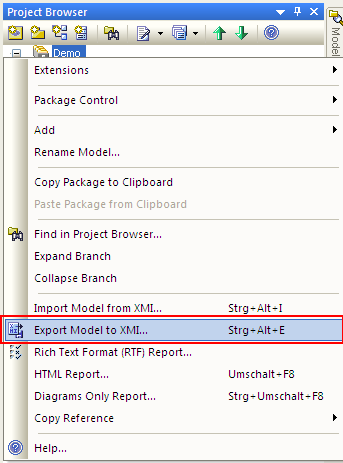
\includegraphics[width=0.5\textwidth]{pics/tricks/projectMigration/projectMigration1}
  \caption{Export the root node from the source EAP}
  \label{fig_projectMigration01}
\end{center}
\end{figure}

\item[$\blacktriangleright$]
Open the target EAP, right-click on the Project Browser and select ``Import Model from XMI...'' (Fig.~\ref{fig_projectMigration03}).
In the dialogue that pops up, enter the name and path of the file to be imported and click \texttt{Import}.

\begin{figure}[htbp]
\begin{center}
  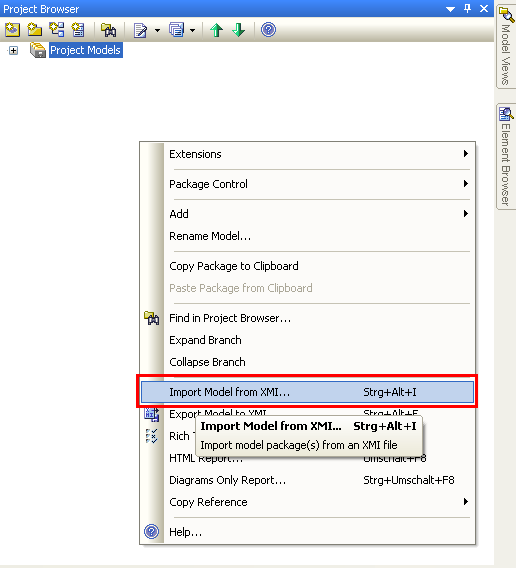
\includegraphics[width=0.5\textwidth]{pics/tricks/projectMigration/projectMigration3}
  \caption{Import the root node into the target EAP}
  \label{fig_projectMigration03}
\end{center}
\end{figure}

\item[$\blacktriangleright$]
After confirming and starting the import, you have to specify how the model should be imported.
As our root models are at the root level, choose ``Yes'' in the dialogue depicted in Fig.~\ref{fig_projectMigration06}.
After the import, you can now delete packages in the root node, which you do not need.
\begin{figure}[htbp]
\begin{center}
  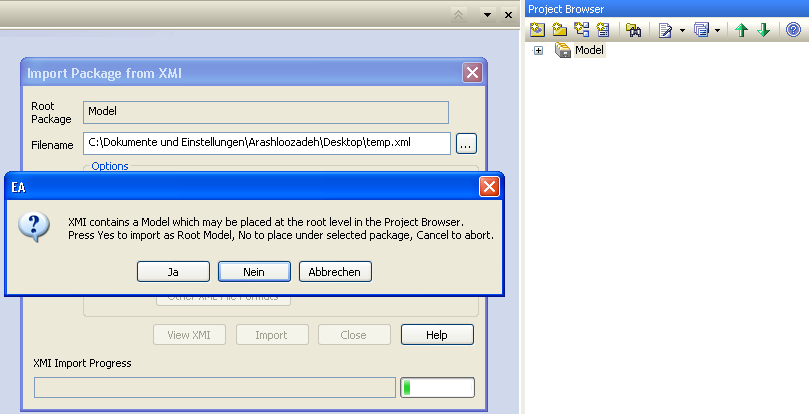
\includegraphics[width=0.5\textwidth]{pics/tricks/projectMigration/projectMigration6}
  \caption{Confirm the level of the root node}
  \label{fig_projectMigration06}
\end{center}
\end{figure}

\end{enumerate}
\clearpage

\section{Using Enterprise Architect with Subversion}
The following steps are required to setup EA for use with subversion.
This is highly recommended when working in a group and sharing a single EA Project (EAP) file, which is otherwise a huge binary blob.
We assume you wish to use (i) Subversion and (ii) Windows.
For other SCM and operating systems please consult the official documentation from EA.

\subsection{Initial preparation and set-up}

Download and install Slik SVN (mandatory):
\begin{enumerate}
  \item[$\blacktriangleright$] x32: \small{\url{http://www.sliksvn.com/pub/Slik-Subversion-1.7.6-win32.msi}}\\\\
   x64: {\small \url{http://www.sliksvn.com/pub/Slik-Subversion-1.7.6-x64.msi}}
\end{enumerate}

For public/private key authentication, you also need Tortoise SVN:

\begin{enumerate}
  \item[$\blacktriangleright$] x32: {\small \begin{minipage}{.95\textwidth}  \url{http://sourceforge.net/projects/tortoisesvn/files/1.7.9/Application/TortoiseSVN-1.7.9.23248-win32-svn-1.7.6.msi/download}
    \end{minipage}}\\\\\\
  x64: {\small\begin{minipage}{.9\textwidth}  \url{http://downloads.sourceforge.net/project/tortoisesvn/1.7.9/Application/TortoiseSVN-1.7.9.23248-x64-svn-1.7.6.msi/download}\end{minipage}}
\end{enumerate}

If you do not want to have your private key password in plain text in an SVN configuration file then also download Pageant:
\begin{enumerate}
  \item[$\blacktriangleright$] {\small \url{http://the.earth.li/~sgtatham/putty/latest/x86/pageant.exe}}
\end{enumerate}

After installing all the tools we need, we now have to setup the SSH tunnel:

\begin{enumerate}
  \item[$\blacktriangleright$] Locate the file \texttt{\%APPDATA\%$\backslash$Subversion$\backslash$config} and open it with your favourite editor. Locate the \texttt{[tunnels]} section.
  \item[$\blacktriangleright$] If you do not want to install Pageant and do not mind entering your password in plain text enter the following command:\\
  \texttt{ssh = "<path to Tortoise SVN>/bin/TortoisePlink.exe" -l \\<username> -pw <password for your private key> -i "<path to your private key>"}
  \item[$\blacktriangleright$] If you wish to use Pageant then the command can be simplified to:\\ \texttt{ssh = "<path to Tortoise SVN>/bin/TortoisePlink.exe" -l \\<username>} as you can add your private key to Pageant.
  \item[$\blacktriangleright$] If you just use direct passwords for authentication then you can leave out the \texttt{-i} option in both cases.
\end{enumerate}

\subsection{How to set-up a version controlled EAP file}
In the following we assume an EAP file has already been placed under version control \emph{according to our tutorial} and that you wish to check-out this file and work with it.
If our instructions do not work, the EAP file might have been placed under version control in a different manner.
If this is the case then please contact whoever checked-in the file and set it up for working with EA and SVN for further instructions.

\begin{enumerate}
  \item[$\blacktriangleright$] Check-out the project with the EAP file from the server using Tortoise-SVN or Eclipse/Subclipse (or any SVN client of your choice).
  You should now have a \textit{.svn}-folder in the directory where you saved the revision.
  \item[$\blacktriangleright$] Open the EAP file.
  If the EAP file is already under version control \emph{and has been set-up correctly}, a dialogue similar to Fig.~\ref{fig:advanced-topics-eaSVN-incompleteConf} should immediately pop-up.
  \item[$\blacktriangleright$] Click ``Yes" to open the ``Version Control Settings'' dialogue (Fig.~\ref{fig:advanced-topics-eaSVN-setWorkingCopyPath}).
\begin{figure}[!htbp]
\begin{center}
	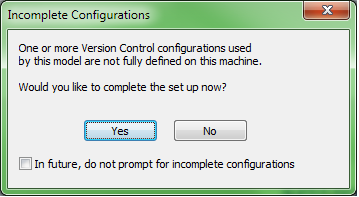
\includegraphics[width=0.5\textwidth]{pics/advancedTopics/eaSVN/DemoLanguages/011}
	\caption{Configure an EAP file which is already under version control}
  	\label{fig:advanced-topics-eaSVN-incompleteConf}
\end{center}
\end{figure}

   \item[$\blacktriangleright$] To work with the EAP file, you now have to \emph{redefine} the SVN variable for the file in your EA workspace.
   To accomplish this, choose the local path to the folder which contains the EAP file in the ``Working Copy Path'' text-box, and correct the value in ``Subversion Exe Path'' if necessary (to fit your Slik installation location).

\begin{figure}[!htbp]
\begin{center}
	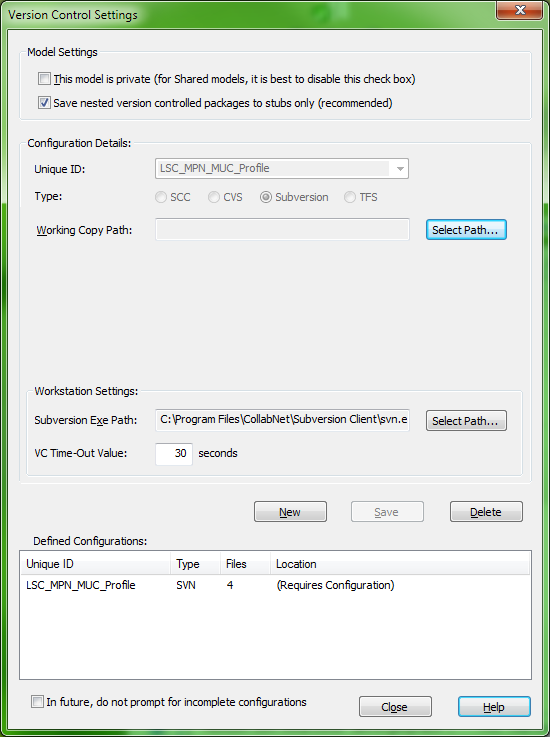
\includegraphics[width=0.5\textwidth]{pics/advancedTopics/eaSVN/DemoLanguages/012}
	\caption{Update settings as required}
  	\label{fig:advanced-topics-eaSVN-setWorkingCopyPath}
\end{center}
\end{figure}

\end{enumerate}

\subsection{Working with a version controlled EAP file}
\label{sect:appendixB_update_commit}

\begin{enumerate}
  \item[$\blacktriangleright$] A \texttt{Check Out} retrieves the lock for a certain package and gives you exclusive access, i.e., no one else can change the package.
  Very important: if subpackages are also under version control, they are not affected by checking out the ``super''-package and remain locked.
  A \texttt{Check Out} also updates the package to the latest version.

\item[$\blacktriangleright$] A \texttt{Check In} commits your work to the server and gives up the lock on the package so others can work on it.
If you do not want to commit your changes, you can just use \texttt{Undo Check Out...} to revert all local changes.

\item[$\blacktriangleright$]  The corresponding \texttt{..Branch} options perform the actions for the current package and all subpackages.
Please note, this has nothing to do with ``branching'' in normal SVN lingo.

\item[$\blacktriangleright$] \texttt{Get Latest/Get All Latest} retrieves the latest version of the selected package / all packages.
This is basically an update but does not retrieve the lock for any package.

\item[$\blacktriangleright$] Conversely, \texttt{Put Latest} saves all your changes without giving up any locks.

\item[$\blacktriangleright$] \texttt{Compare with controlled version} can be used to review incoming changes.
Green elements will be added, red will be deleted.

\item[$\blacktriangleright$] \texttt{File History} gives you a summary of all commits made while you were lying on the beach.
For a useful file history, always use meaningful commit statements when checking in!
A date stamp is created automatically.
\end{enumerate}

\subsection{Placing an EAP file under version control}
\label{sect:appendixB_new_EAP_for_vc}

If you already have an EAP file and would like to place it under version control, you first have to check it in as usual on the server using your favourite SVN client.
Once the project is checked in, the required .svn folder should be in the folder containing the EAP file.
The next step is to register an SVN-variable in EA:
\begin{enumerate}
  \item[$\blacktriangleright$] Open the EAP file, right click on a root folder and select ``Package Control'' and then ``Version Control Settings...'' (Fig.~\ref{fig:advanced-topics-eaSVN-rightclick}).
\begin{figure}[!htbp]
\begin{center}
 	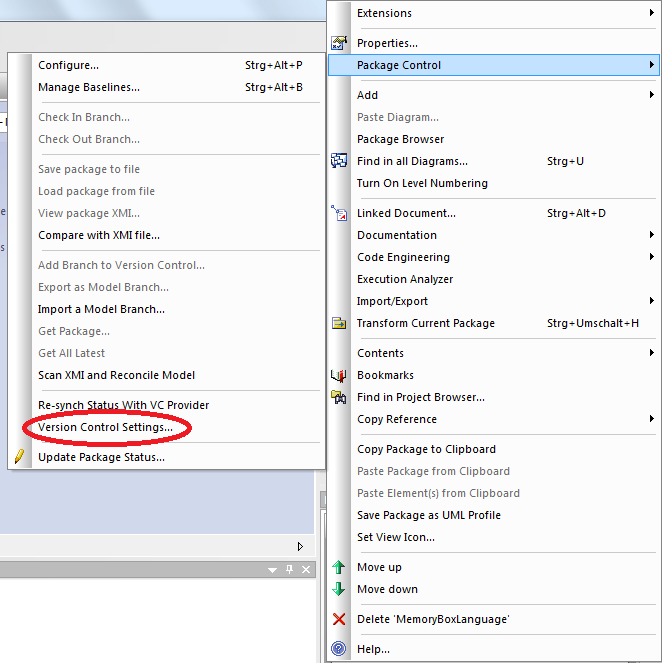
\includegraphics[width=0.7\textwidth]{pics/advancedTopics/eaSVN/rightclick}
	\caption{Select version control settings}
  	\label{fig:advanced-topics-eaSVN-rightclick}
\end{center}
\end{figure}
  \item[$\blacktriangleright$] In the dialogue, choose a unique ID of your choice (we suggest you use the name of the EAP file) for the settings and activate the ``Subversion'' radio button below.
  \item[$\blacktriangleright$] Choose the local path to the folder which contains the EAP file in the ``Working Copy Path'' text-box.
  \item[$\blacktriangleright$] The field ``Working Station'' must point to where you installed Sliksvn, i.e., \texttt{<path to SlikSVN>$\backslash$bin$\backslash$svn.exe")}.
  Press ``Save'' and close the dialogue (Fig.~\ref{fig:advanced-topics-eaSVN-variable}).
  If the dialogue closes without an error message, then you can be sure to have configured everything correctly.
%\usepackage{graphics} is needed for \includegraphics
\begin{figure}[!htbp]
\begin{center}
	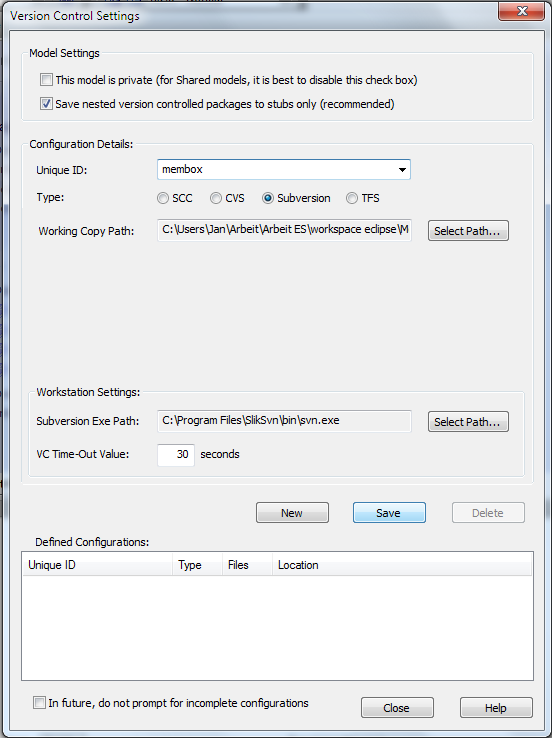
\includegraphics[width=0.6\textwidth]{pics/advancedTopics/eaSVN/versioncontrol}
	\caption{Register an SVN variable in EA}
  	\label{fig:advanced-topics-eaSVN-variable}
\end{center}
\end{figure}
\item[$\blacktriangleright$] In the EAP file, choose ``Package Control$\backslash$Configure...'' for \emph{each package} you wish to place under version control.

\item[$\blacktriangleright$] In the ensuing dialogue, activate ``Control Package'' and select your previously defined SVN variable from the drop-down menu.
Enter the path where the XML file for the project should be placed.
Although this is not enforced in any way, we recommend you create a folder structure that mirrors the package structure in EA (Fig.~\ref{fig:advanced-topics-eaSVN-addPackage}).
This process has to be repeated \emph{for all sub-packages} as soon as their super-package has been placed under version control.
\begin{figure}[!htbp]
\begin{center}
	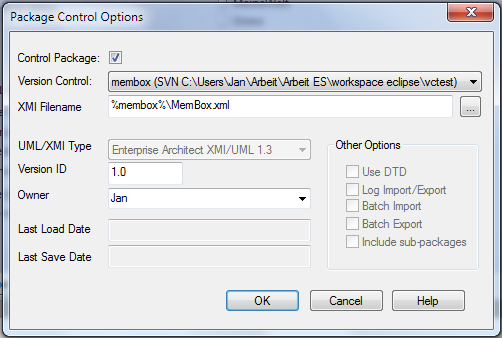
\includegraphics[width=0.6\textwidth]{pics/advancedTopics/eaSVN/cont}
	\caption{Placing a package under version control}
  	\label{fig:advanced-topics-eaSVN-addPackage}
\end{center}
\end{figure}

\item[$\blacktriangleright$] As a final step, check-in the current state of the EAP file directly with your SVN client.
As from this point, the EAP file should not be checked-in anymore, and all versioning actions should be performed via EA (and not directly with your SVN client).
\end{enumerate}
\clearpage

\section{Conditional branching with StatementNodes}

When working with SDMs, you often need to choose between two different patterns based on the return value of an arbitrary (black box) operation.
This is like the normal \texttt{Success}/\texttt{Failure} construction, but instead of a pattern being matched or failing, the decision can be implemented with a another SDM or a standard Java method.
This feature is a further means (besides \texttt{MethodCallExpressions} for attribute values and \texttt{Bindings}) of integrating hand-written Java code in SDMs (and can lead to spaghetti SDMs so please use with caution!).

As an example, consider a class \texttt{A} with an operation:
\begin{quote}
 \mbox{\texttt{doSomeCheck(p$_1$,\ldots,p$_n$ :EClass) :EBoolean}}
\end{quote}

This method could be implemented in hand-written Java code or be specified by another SDM specification.

Although dummy boolean attributes \emph{could} be used to achieve the same effect, it is much simpler to branch the control flow based on the result of a \texttt{StatementNode}.
If the method returns an \texttt{EBoolean}, \texttt{Success} and \texttt{Failure} correspond to \texttt{true} and \texttt{false}, respectively.
If the method returns anything else, then \texttt{Failure} corresponds to \texttt{null}.
Void methods \emph{cannot} be used to branch and an exception is thrown during code generation.

Fig.~\ref{fig:cond_branch_on_op} depicts the class \texttt{A} and shows how \texttt{doSomeCheck} is used to branch in an SDM.
Fig.~\ref{fig:cond_branch_on_op_code} depicts the corresponding generated if/else branch in Java.

\begin{figure}[htp]
\begin{center}
  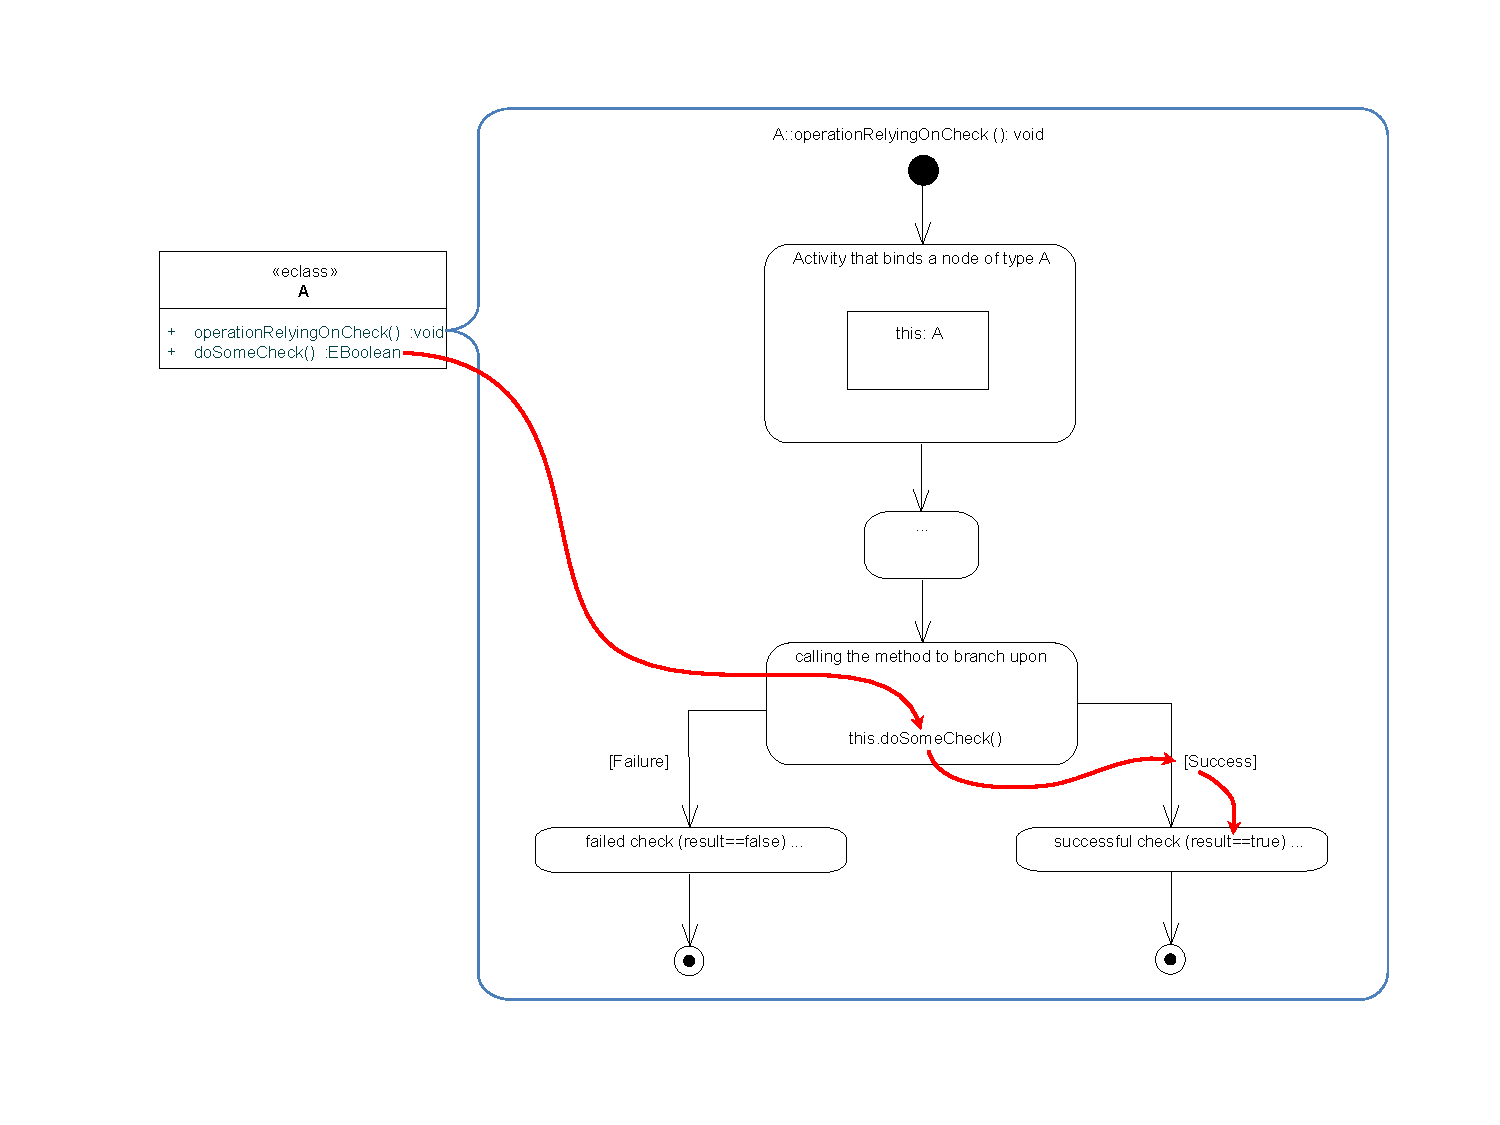
\includegraphics[width=1\textwidth]{pics/advancedTopics/branching/SDM_with_branch}
  \caption{Conditional branching based on the result of an operation}
  \label{fig:cond_branch_on_op}
\end{center}
\end{figure}

\begin{figure}[htp]
\begin{center}
  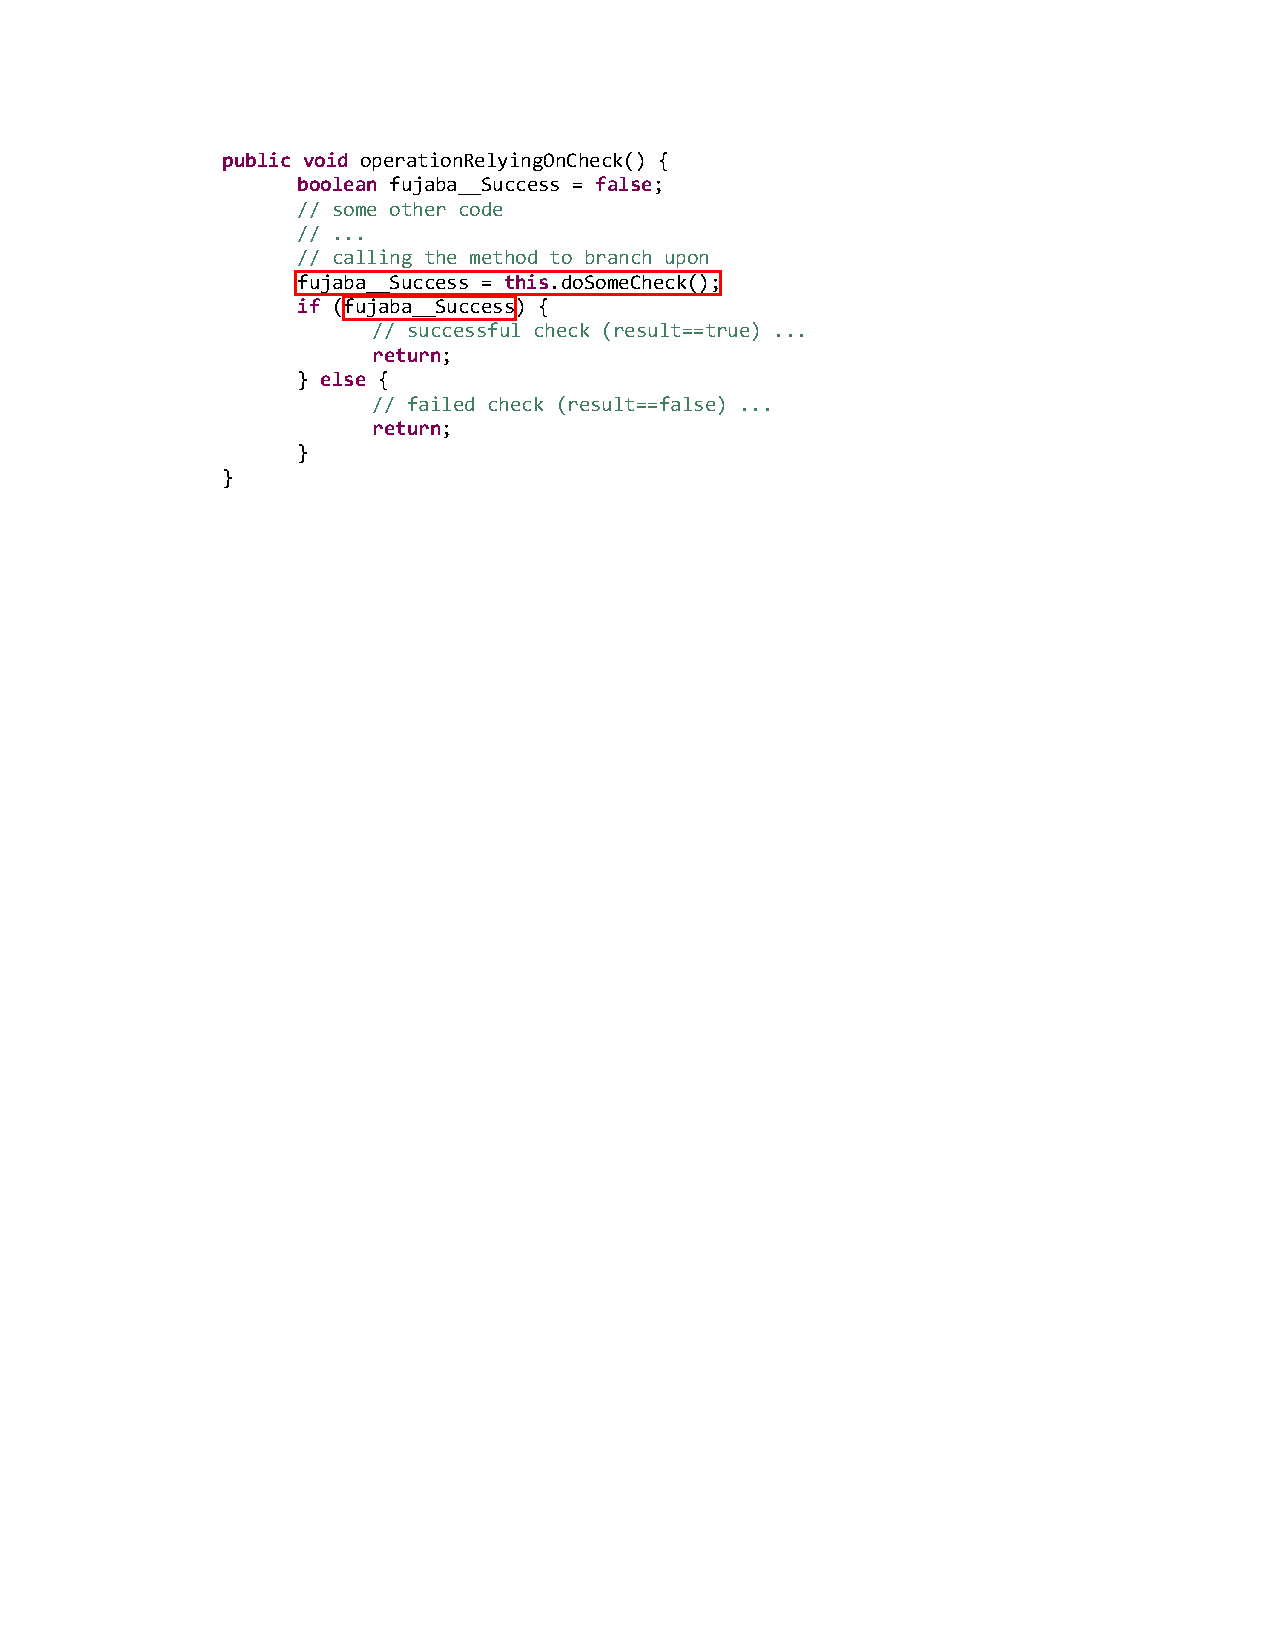
\includegraphics[width=0.7\textwidth]{pics/advancedTopics/branching/generated_code}
  \caption{Generated code for branch}
  \label{fig:cond_branch_on_op_code}
\end{center}
\end{figure}

Perform the following steps to branch with a \texttt{StatementNode}:
\begin{enumerate}
\item[$\blacktriangleright$] Add a new statement node (cf.~Fig.~\ref{fig:cond_statement_node}) at the appropriate location in your SDM.
\item[$\blacktriangleright$] Invoke a non-void method (an operation in the metamodel) via a \texttt{MethodCallExpression} (cf.~Fig.~\ref{fig:cond_method_call}).
\item[$\blacktriangleright$] Add \texttt{Success} \emph{and} \texttt{Failure} edges to the \texttt{StatementNode} to branch appropriately.
\end{enumerate}

\begin{figure}[htp]
\begin{center}
  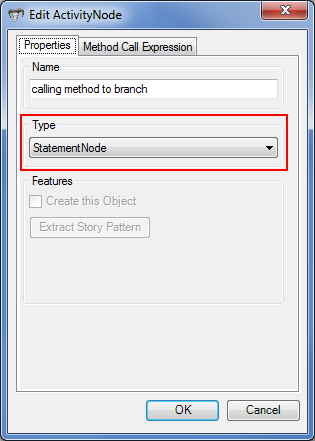
\includegraphics[width=0.5\textwidth]{pics/advancedTopics/branching/01_switch_to_statement_node}
  \caption{Switch from activity node to statement node}
  \label{fig:cond_statement_node}
\end{center}
\end{figure}

\begin{figure}[htp]
\begin{center}
  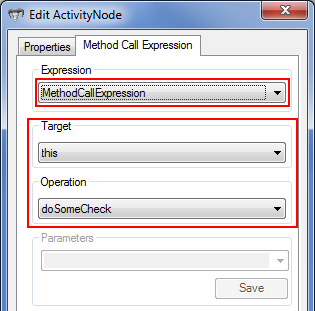
\includegraphics[width=0.5\textwidth]{pics/advancedTopics/branching/02_specify_method_call_expression}
  \caption{Specify the method call expression}
  \label{fig:cond_method_call}
\end{center}
\end{figure}

\clearpage

% \section{Preserving files on Clean}

% Although the EMF code generator tries its best to merge hand-written and generated code (and does a pretty good job!), you will still need to \emph{Clean and Build} now and then.

% To support this, we have a naming convention to indicate classes with hand-written code (which should not be deleted on a clean):
% \begin{quote}
% All files with ``\ldots \texttt{.facade.impl.}\ldots'' in their path are automatically preserved when cleaning\ldots
% \end{quote}

% If you place your helpers in a package named \texttt{*facade*}, therefore, the corresponding \texttt{*impl} files (where you can implement the methods by hand) will be preserved automatically.

% In some cases, it might be necessary to mark additional files or folders that do \emph{not} follow this naming convention but should nonetheless be preserved when cleaning.

% To do this, we provide the following options (Fig.~\ref{fig:preservepath}):
% \begin{itemize}
% \item [$\blacktriangleright$] To add a file or folder to the list of \emph{preserved paths}, right click on the file or folder to invoke the context menu and choose\\ \mbox{\texttt{eMoflon} $\rightarrow$ \texttt{Add to preserve path}}.

% When a folder is specified, \emph{all folders and paths with this path as prefix} are preserved.
% \item [$\blacktriangleright$]To remove a path that is already on the list, choose\\ \mbox{\texttt{eMoflon} $\rightarrow$ \texttt{Remove from preserve path}}.
% \end{itemize}

% Paths to be preserved are added to the \texttt{PRESERVE\_PATHS} variable in the \texttt{moflon.properties} file of the corresponding eMoflon project.

% All paths are created relative to the Eclipse workspace, i.e., are of the form:
% \texttt{/<ProjectName>/gen/<Path>/<File>}.
% \clearpage

% \begin{figure}[htp]
% \begin{center}
%   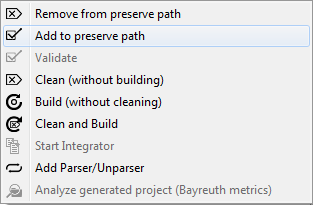
\includegraphics[width=0.5\textwidth]{pics/advancedTopics/preservePath/PreservePath}
%   \caption{eMoflon context menu}
%   \label{fig:preservepath}
% \end{center}
% \end{figure}
